\documentclass[a4paper,10pt]{article}
\usepackage[utf8]{inputenc}
\usepackage{graphicx}
\usepackage{float}
\usepackage{subfig}
\usepackage[square,numbers]{natbib}
\bibliographystyle{unsrtnat}

\title{Ray Tracing Through The Graphics Pipeline\\ 
 EEC 277 Final Project}
\author{Ahmed H. Mahmoud and Yuxin Chen}

\begin{document}

\maketitle

\section{Introduction}
The reason we can see objects because photons are reflected into our eyes basing on the observation: firstly, without light we cannot see anythiny and secondly, withou object in our environment, we cannot see light. If we were to travel in intergalactic space, if there is no stuff around us, we cannot see anything but darkness even though photons are potentially moving through that space. This gives us (the old researchers) the idea that we can produce a picture by simulating the behavior of photons emitted by light sources, then there is another physical phenomena which we need to be aware of. Comparing to the total number of rays reflected by an object, only a select few of them will ever reach our eyes. So we would potentially have to cast zillions of photons from the light source to find only one photon that would strike the eye. This approach is called forward ray-tracing. Thus forward ray-tracing requires a computation power which is impossible in that age maybe also impossible in this age. Then Turner Whitted \cite{whitted2005improved} came, solving this problem together with reflection, refraction, shadows and hidden surface removal by the way by backward ray tracing which tracks the ray backwards from eye to the object. Then it saves tons of computation of photons which finally do not get to our eyes, making ray racing possible. Also because it integrates reflection, refraction, hidden surface removal and shadows into one model, ray tracing is thus regarded as a versatile rendering technique for light-object interaction. It is something value worth research's time.
\section{Why Graphics Pipeline}
In order to speed up the computation of ray tracing, one can implemented it in parallel where each ray computation is done independently. A natural choice to carry out such computation is a general purpose API such as CUDA. But such APIs could be limited to a specific vendor which limit the usability of such program. Due to the wide spread of the graphic pipeline implementation and hardware support across different systems, we can guarantee the reliability of the program on various operating systems and GPUs. 

Nowadays, ray tracing applications are not confined to desktop applications. Web browsers (using WebGL) and mobiles (using OpenGL ES) applications are now on the rise. Exploring the graphics pipeline applicability to perform ray tracing would be attractive for such systems. This is due to the close matching between OpenGL and OpenGL ES and WebGL, since they both are limited version of OpenGL \cite{hachisuka2015implementing}.

There are certain challenging to perform such a general-purpose program through the fixed graphics pipeline. For example, OpenGL Shading Language (GLSL) does not support recursion, pointers, or self referential struct which are all a handy tools for any programmer. The fixed pipeline requires passing through different stages that might not be necessary for the computation for ray tracing. 

\section{Implementation Details}
Here we list the major steps towards the implementation of brute force ray tracing for a static scene. We initialize the scene as two triangles such that the vertex shader just outputs the position of each vertex with minimal/no computation. All the computation takes place in the fragment shader. For each pixel, a ray is shot towards the scene. In order to calculate different effect such as reflection and shadow, a ray should bounces multiple times in order to get the effect correctly. Due to lack of recursion support, a certain depth for number of bounces a ray can do should be declared beforehand. We set this number to 5. We used spheres as our primitives but the same computation can be carried out using triangles. For the brute force implementation, each ray was tested against all objects in the scene. 

\subsection{Use of Texture Memory}
In order to move the scene objects from the application to the graphics pipeline, one would have to pass these objects all the way down the pipeline until the fragment shader start execution. We started by using \emph{uniform} type qualifier since it is a read-only, fast, do not have to change from one execution of shader program to the next which makes it excellent for our purpose. We used them to test trivial scenes ($\leq 100$ spheres). OpenGL has only very limited number of uniform that can be declared which forced us to detach them. 

We explored two options to use the texture memory; Image Load/Store Texture and Shader Storage Buffer Objects (SSBO). We chose to use SSBO because it allows use of interface block such that we can define variable of different types (int, float, arrays, etc) which is typical for our purpose. Additionally, SSBO can offer upto the size of the GPU memory and it can have unbounded storage (up to the buffer range bound). In contrast, texture image allows only vec4 or combination of them. Also, read and write from texture was complex, unlike binding to SSBO and read from it. Another options could have been Uniform Buffer Objects (UBO), but they suffer from limitation over the size that can be used. UBO also should have specific, fixed storage size at compile-time. 

\begin{figure}[!tbh]
 \centering     
   \subfloat [Bunny]{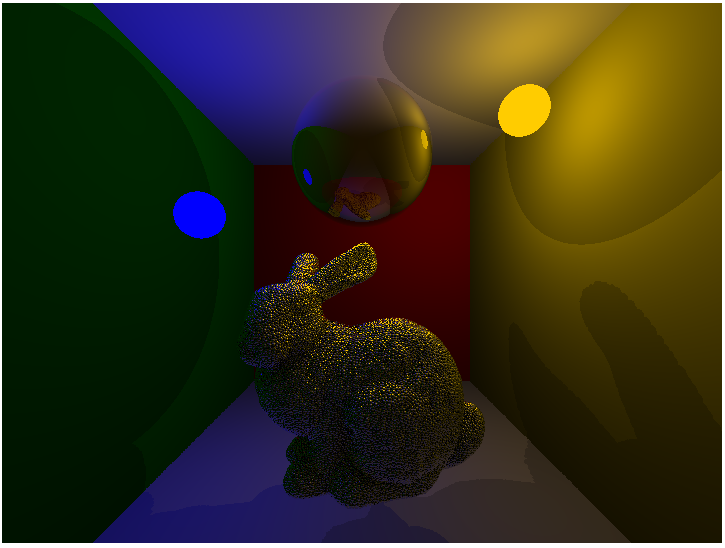
\includegraphics[width=0.3\textwidth]{bunny.png}}
   \subfloat [Fertility]{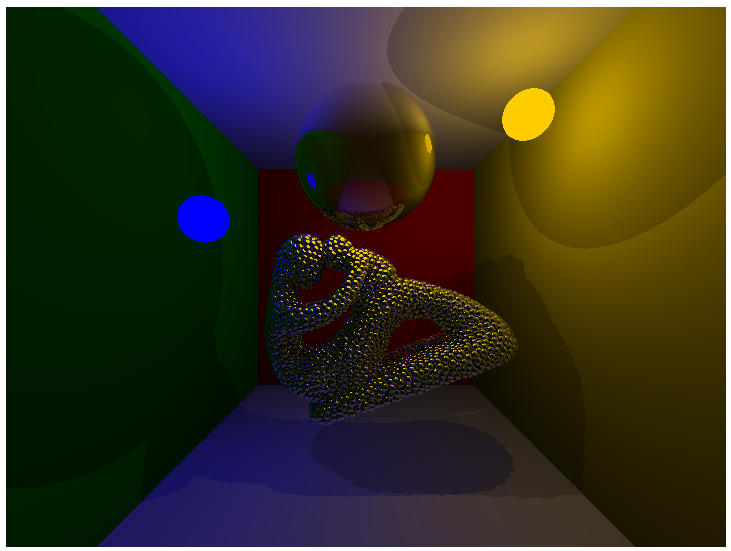
\includegraphics[width=0.3\textwidth]{fertility.png}}
   \subfloat [Sphere]{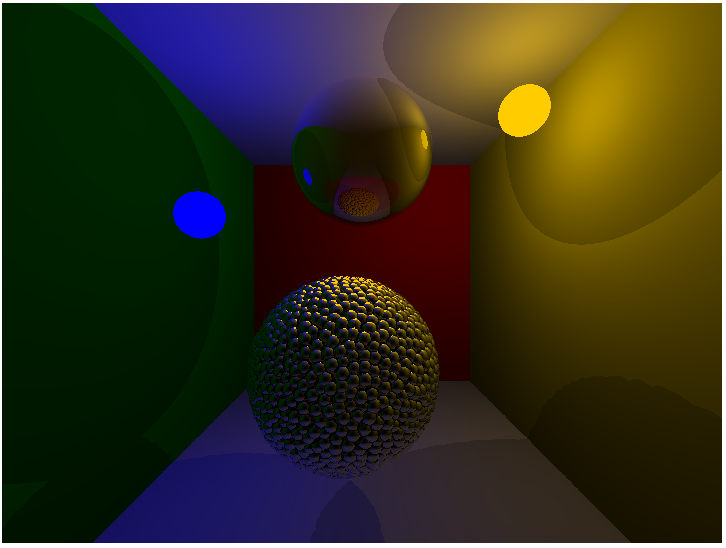
\includegraphics[width=0.3\textwidth]{sphere.png}}   
   \subfloat [Torus]{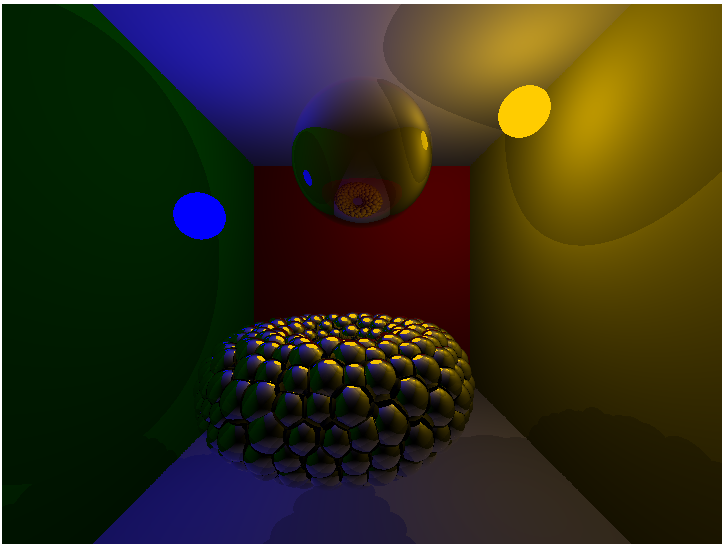
\includegraphics[width=0.3\textwidth]{donut.png}}
   
     \caption{Results of brute-force ray tracing}
   \label{fig:brute}
\end{figure} 
   
   
\section{Acceleration Structure: Bounding Volume Hierarchy}
In \cite{whitted2005improved} Whitted estimated that a recursive ray tracer spends up to 95\% of its time testing for intersections. This imposes a huge computational cost to the process. There are two aspect in terms of the high cost for intersection checks. 
\begin{enumerate}
    \item Intersection checks for every objects. If the number of objects are high, this process can be painful even if most of objects end up not intersecting with the ray.
    \item Computational expense of each intersection test depends on the complexity of the object representation. 
\end{enumerate}
One approach resolving the second issue is using bounding volume with intersection checks. If a ray does not intersect the bounding volume of an object, then the object is ignored from further processing for that particular ray. We are using axis-aligned bounding boxes(AABBs) which only require simple (basically compare) and small number of operation for intersection check. However, one point worthy mention: usually the tighter the bounding box fits the object, them few of the rays intersecting this bounding volume are likely to actually miss the object inside. However, if the bounding box has a complex shape, then it increase the cost for intersection check. Obviously, the bounding volume that fits this criteria is the object itself. A good choice for a bounding volume is therefore a shape that provides a good trade-off between tightness and speed. \\
To address the first issue, an intuitive method is to only check subset of object who are likely be intersected. We build our approach around a bounding volume hierarchy, where each group is associated with a conservative bounding box. 
\begin{figure}[H]
    \centering
    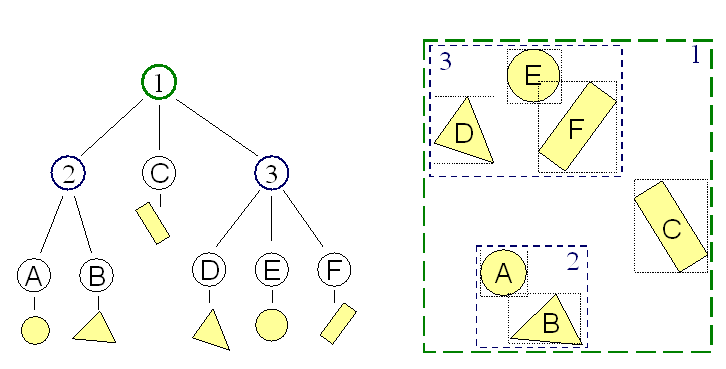
\includegraphics[scale=0.3]{bvh.png}
    \caption{Example of bounding volume hierarchy}
    \label{fig:bvh}
\end{figure}
Effective use of BVH tree can be explain further into two aspects:
\begin{enumerate}
    \item Efficient tree traversal ?? efficient or effective? 
    \item Effective construction of BVH tree
\end{enumerate}
The explanation about first issue is discussed more in other Optimization since it is related more on how to minimize divergence on data and instruction. We will mainly talk about how to construct BVH tree in parallel in this section. \\
Why construction speed is of the essence? Suppose we use ray tracing in game or physics simulation, each frame, the objects can move, thus requiring a different BVH for each frame. So it is nontrivial to build the BVH tree fast. \\
The most promising parallel BVH construction approach is to use a so-called linear BVH(LBVH). The idea is to simplify the problem by first choosing the order in which the leaf nodes appear in the tree, and then generating the internal nodes in the a way that use this order. For data locality consideration, we prefer the objects that located close to each other in 3D space to also reside nearby in the hierarchy since objects nearby are highly checked together and data can happen to be preloaded in the memory because cache line is the base unit loaded. So a reasonable choice is to sort them using their Morton codes which encoding the space position information within the code. Then use parallel radix sort is the right tool for this job. A good way to assign the Morton code for a give object is to use the centroid point of its bounding box. Then we can sort those objects by their space position information and generate a node hierarchy where each subtree corresponds to a linear range of sorted primitives so that ones close to each other in 3D end up close to each other in the resulting tree. \\
Then we use the method describe in \cite{karras2012maximizing} to parallel construct the binary radix tree. One key insight in enabling parallel construction is to establish a connection between node indices and keys through a specific tree layout. The idea is to assign indices for the internal nodes in a way that enables finding their children without depending on earlier results. Using Morton code, we can easily know give a range how should we cut the range and make it into a tree. Then problem becomes how to find the range independently. We can take the advantage that the index of very internal node coincides with either its first or its last key. Then what you need to find out which direction it tends to be on the tree and its upper bound or low bound by comparing the length of the prefix with other objects (a larger difference on the prefix indicate it is likely to cut at this point). Nicely, the time complexity of this algorithm in the worst case is $\mathcal{O}(n\log_n)$.

\subsection{Tree Traversal:}



\medskip

\bibliography{sample}

\end{document}
